% ====================================================================================================
% SECTION 1  INTRODUCTION  (budget ~0.9 page)
%   Motivation -> task (quality estimation, not splitting) -> approach (Figure 1) -> RQ1/RQ2 -> contributions.
% ====================================================================================================

\section{Introduction}
\label{sec:intro}

Sentence segmentation is the first step of most NLP pipelines, and its errors propagate into parsing, translation and
retrieval. Segmenters differ in how they work---unsupervised abbreviation statistics in Punkt
\citep{kiss-strunk-2006-unsupervised}, supervised taggers trained on treebanks in Stanza \citep{qi-etal-2020-stanza},
punctuation-agnostic transformers in WtP and SaT \citep{minixhofer-etal-2023-wheres,frohmann-etal-2024-segment}---and
they behave differently across domains \citep{read-etal-2012-sentence}. A segmenter that is nearly perfect on news can
fail on forum posts without punctuation, on headlines or on lists. Yet whoever applies a segmenter to a new domain
usually has no gold boundaries with which to check its output.

We study \emph{reference-free quality estimation} for sentence segmentation: given raw text and a segmenter's output,
estimate the output's quality without gold boundaries for the target domain. This is a different task from
\emph{splitting}. A splitter must produce boundaries; a quality estimator judges an existing segmentation and can be used
to compare segmenters, to flag badly segmented documents, or to choose a segmenter for a new domain. Gold boundaries of a
source corpus (here GUM) may be used for training; target-domain gold is used only to validate the estimator.
Reference-based metrics---boundary precision, recall and F1, $P_k$, WindowDiff---cannot be computed in this setting.
Reference-free quality estimation is established for machine translation \citep{specia-etal-2018-quality}, but it is
underexplored for segmentation, so we also have to answer a second question: \emph{how should such an estimator be
evaluated?}

Our evaluator (Figure~\ref{fig:overview}) has two parts. It first predicts a boundary probability $p_i$ at every gap
between words, fusing techniques from the course \citep{jurafsky-martin-slp3}---regular-expression rules, a Kneser--Ney $n$-gram
model, a maximum-entropy probe---with pretrained neural boundary models; the fusion is trained on GUM so that the resulting scores
track true quality. It then scores a candidate segmentation by its \emph{normalized Soft F1} against these
probabilities, a score that is comparable across documents and well defined for documents with a single sentence. We ask:

\begin{description}
  \setlength\itemsep{0pt}
  \item[RQ1] Can a reference-free score rank real segmentation outputs by their true quality on held-out data,
  and how does it compare with the evaluators a practitioner would naturally try? (\S\ref{sec:rq1})
  \item[RQ2] Which segmentation errors does it notice, and what limits its reliability?
  (\S\ref{sec:rq2a}--\ref{sec:rq2b})
\end{description}

\noindent Our contributions are:
\begin{enumerate}
  \setlength\itemsep{0pt}
  \item \textbf{Method} (\S\ref{sec:method}): a reference-free quality estimator for sentence segmentation that fuses
  probabilistic boundary evidence---rules, a Kneser--Ney trigram model, a maximum-entropy probe on frozen BERT, zero-shot
  SaT and a fine-tuned boundary tagger---and scores an existing segmentation by normalized Soft F1 with a document-end
  correction.
  \item \textbf{Evaluation design} (\S\ref{sec:eval}): three views---agreement with true quality, the ranking of
  segmenters, and sensitivity to specific error types with a quality-neutral control---against nine baselines (rules,
  language models, a strong segmenter used as pseudo-reference or as evidence, multi-system consensus); gold isolation and
  pre-registered one-shot tests of the final evaluator on new held-out splits.
  \item \textbf{Findings} (\S\ref{sec:results}): on the fresh EWT dev split the evaluator reaches Spearman $\rho = 0.797$,
  $+0.141$ [$+0.075$, $+0.213$] over system consensus (0.851 given paragraph structure), on par with the strongest
  supervised segmenter plugged into the same scoring ($+0.035$, n.s.). Error injection shows complementary blind spots
  and the limits of transfer across annotation conventions.
\end{enumerate}

\begin{figure*}[t]
  \centering
  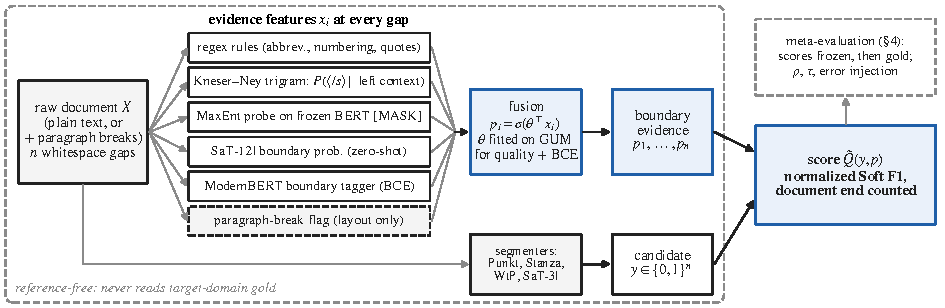
\includegraphics[width=\textwidth]{figures/f1_overview.pdf}
  \caption{The evaluator. Every source of evidence reads only the raw document; their features are fused into a
  boundary probability $p_i$ per gap, and each candidate segmentation is scored against $p$ by normalized Soft F1
  (\S\ref{sec:scoring}). Gold of the evaluated corpus is read only after all scores are frozen (\S\ref{sec:protocol}).
  The paragraph-break flag is used only in the controlled ``paragraphs given'' condition (\S\ref{sec:data}).}
  \label{fig:overview}
\end{figure*}
